\section{Continuidad}

\begin{defn}[Continuidad\IS en un punto]
Sea $\appl{f}{D\subset\real}{\real}$.

Se dice que $f(x)$ es continua en $x=a$ sí y solo si se cumplen las 3 condiciones siguientes:
\begin{itemize}
	\item $\exists \displaystyle\lim_{x\to a} f(x)$
	\item $\exists f(a)$
	\item $\displaystyle\lim_{x\to a}f(x) = f(a)$
\end{itemize}

\textit{También se puede decir de manera abreviada: \[f(x) \text{ continua en } x=a\dimplies \text{ existen y son iguales } \lim_{x\to a}f(x) \text{ y } f(a)\]}
\end{defn}

\begin{problem}
Halla el valor de $m$ para que la función sea continua en $x=0$.
\[f(x) = 
	\begin{cases}
		2x-5 & \text{ si }x\leq 0\\ 
		\frac{2x+m}{x+1} & \text{ si } x>0
	\end{cases}\]
\solution

Aplicamos: "$f(x)$ continua en $x=0$ si existen y son iguales $\displaystyle\lim_{x\to 0}$ y $f(0)$".

\begin{itemize}
	\item $f(0) =  2·0-5 = -5$
	\item $\displaystyle\lim_{x\to0} f(x)$. Para calcularlo necesitamos los límites laterales:
	\subitem $\displaystyle\lim_{x\to0^+} f(x) = \lim_{x\to0^+} \frac{2x+m}{x+1} = \frac{2·0+m}{0+1} = m$
	\subitem $\displaystyle\lim_{x\to0^-} f(x) = \lim_{x\to0^-} 2·x-5 = -5$

	\[\exists\lim_{x\to0}f(x) \dimplies \lim_{x\to 0} f(x) = -5 \dimplies m=-5 \text{ porque } \begin{cases}\displaystyle\lim_{x\to0^+}f(x) = m\\ \displaystyle\lim_{x\to0^-}f(x) = -5\end{cases}\]
	\item Si $m=-5$, $f(x)$ es continua en $x=0$.
\end{itemize}

\end{problem}

\paragraph{Tipos de discontinuidad}

\[
\begin{cases} 
	\text{Continua}\\
	\text{ Discontinua }
		\begin{cases}
			\text{Evitable}\\
			\text{Esencial}
				\begin{cases}
					\text{1ª especie}
						\begin{cases}
							\text{Salto finito}\\
							\text{Salto infinito}
						\end{cases}\\
					\text{2ª especie}
				\end{cases}
		\end{cases}
\end{cases}
\]


\textbf{Descripción: } Libro página 22. 
\begin{itemize}
	\item Evitables: $\exists \displaystyle\lim_{x\to a}f(x)$ pero $\begin{cases}\displaystyle\lim_{x\to a}f(x) \neq f(a)\\\text{o}\\\nexists f(a)\end{cases}$. Ejemplo: 
	\subitem Para evitarlas, \quad\quad\quad\quad una nueva función: $f(x) = \begin{cases}f(x) & x\neq a\\ \displaystyle\lim_{x\to a}f(x) & x=a \end{cases}$
	\item Esenciales (o inevitables): 
	\begin{itemize}
		\item De primera especie:
		\subitem De salto finito: ambos límites laterales son finitos pero distintos. Ejemplo:
		\subitem De salto infinito: al menos un límite lateral es infinito. Ejemplo:
		\item De 2ª especie: al menos un límite lateral no existe. Ejemplo:
	\end{itemize}
\end{itemize}


\begin{figure}[hbp]
\centering
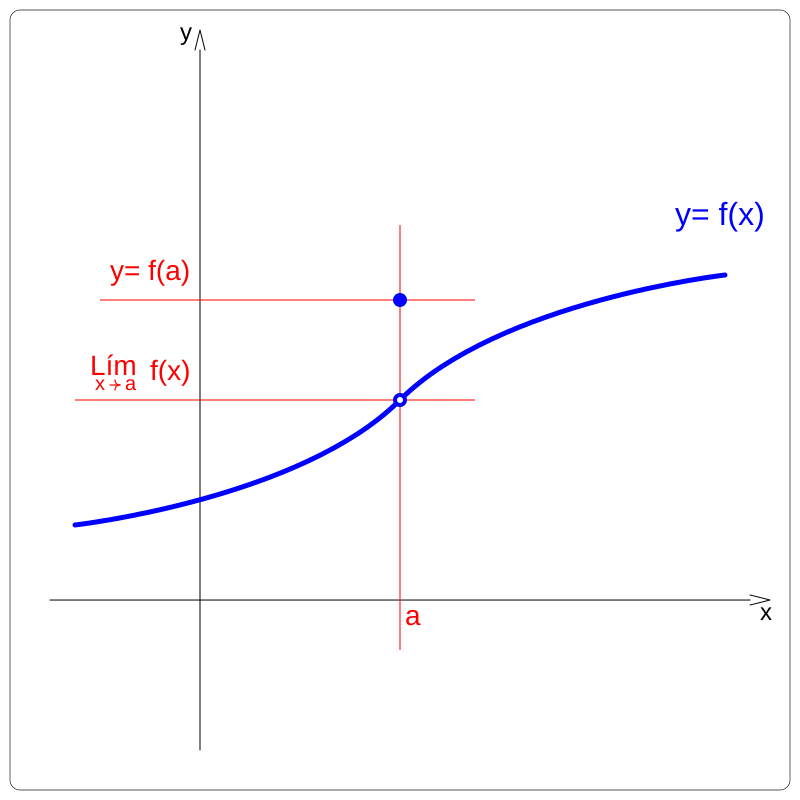
\includegraphics[scale=0.195]{img/Funs/funcion_xy_discontin_4hStg}
%\caption{Ejemplo de discontinuidad evitable}
\label{fig::fun-tipos-discontinuidad}
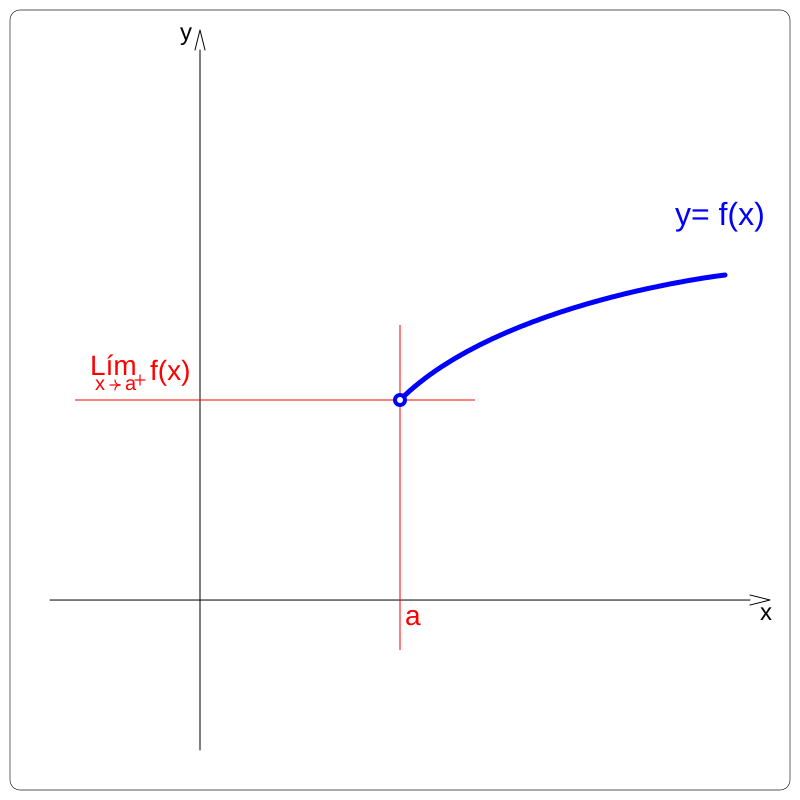
\includegraphics[scale=0.195]{img/Funs/funcion_xy_discontin_4jSGg}
%\caption{Ejemplo de discontinuidad de }
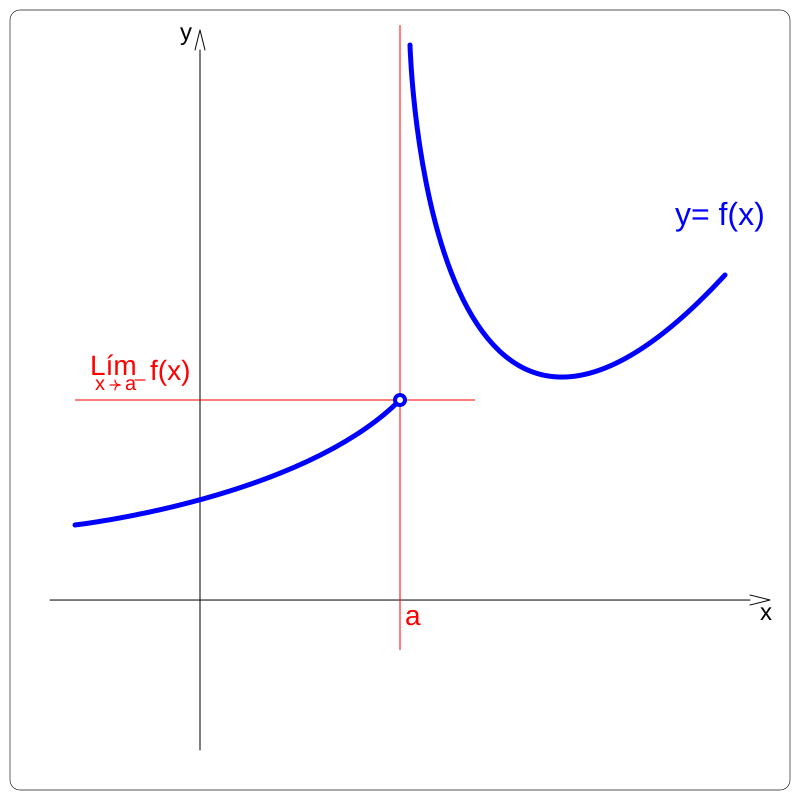
\includegraphics[scale=0.195]{img/Funs/funcion_xy_discontin_6ueR5}
%\caption{Ejemplo de discontinuidad de }
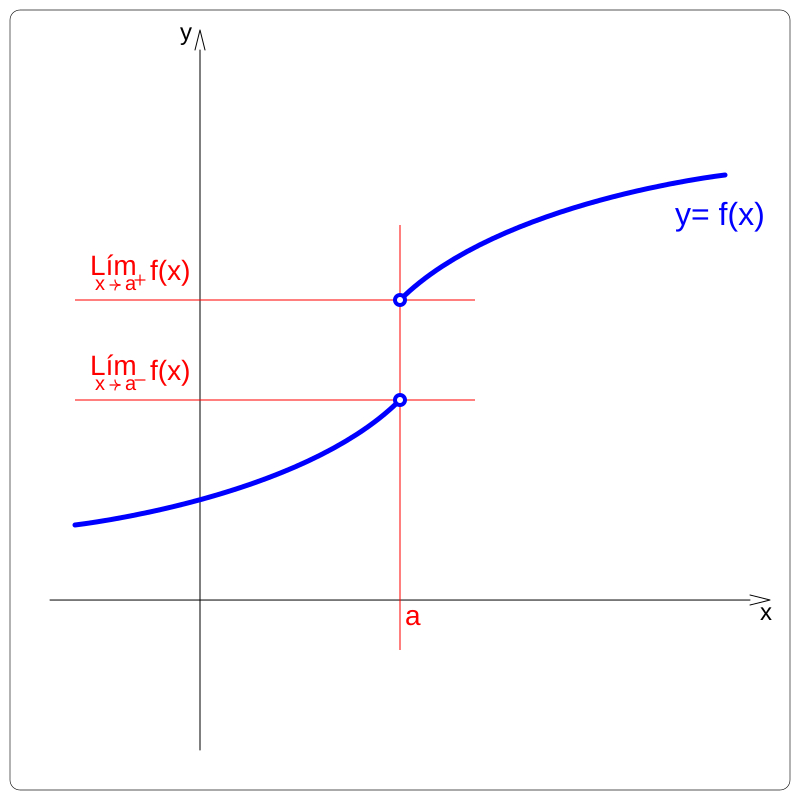
\includegraphics[scale=0.195]{img/Funs/funcion_xy_discontin_U72G2}
%\caption{Ejemplo de discontinuidad de }
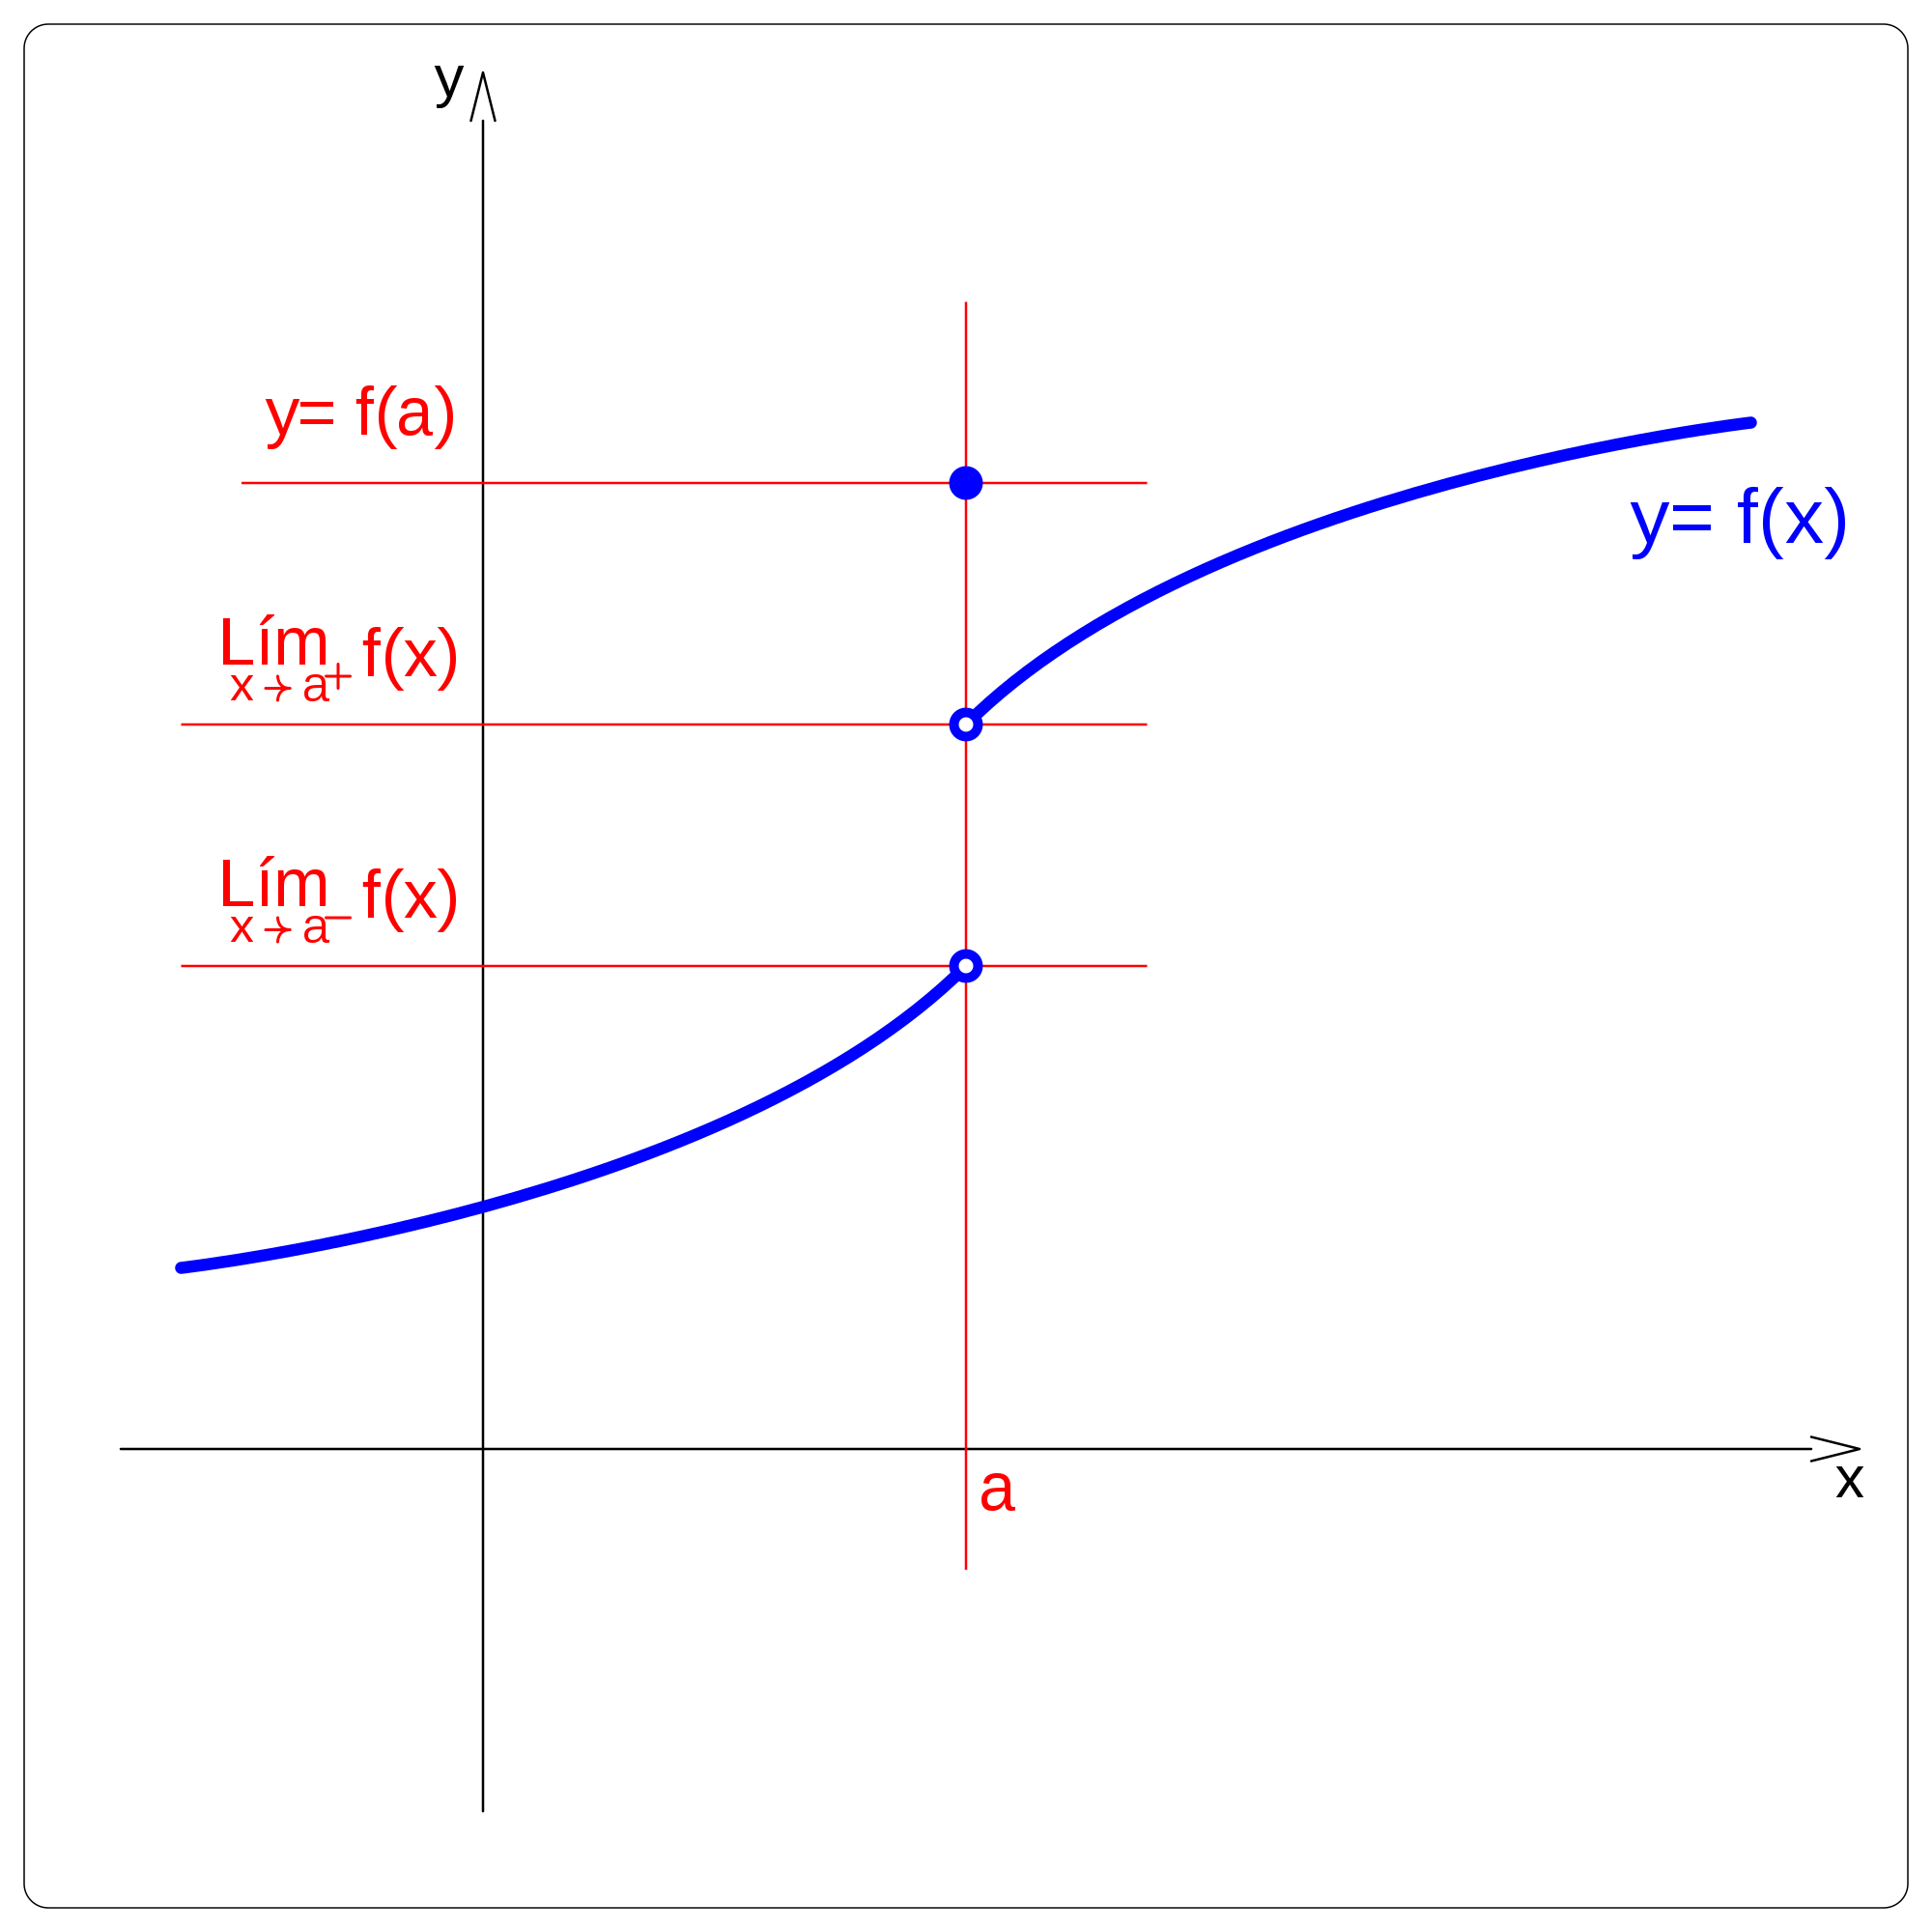
\includegraphics[scale=0.06]{img/Funs/2f2}
%\caption{Ejemplo de discontinuidad de }
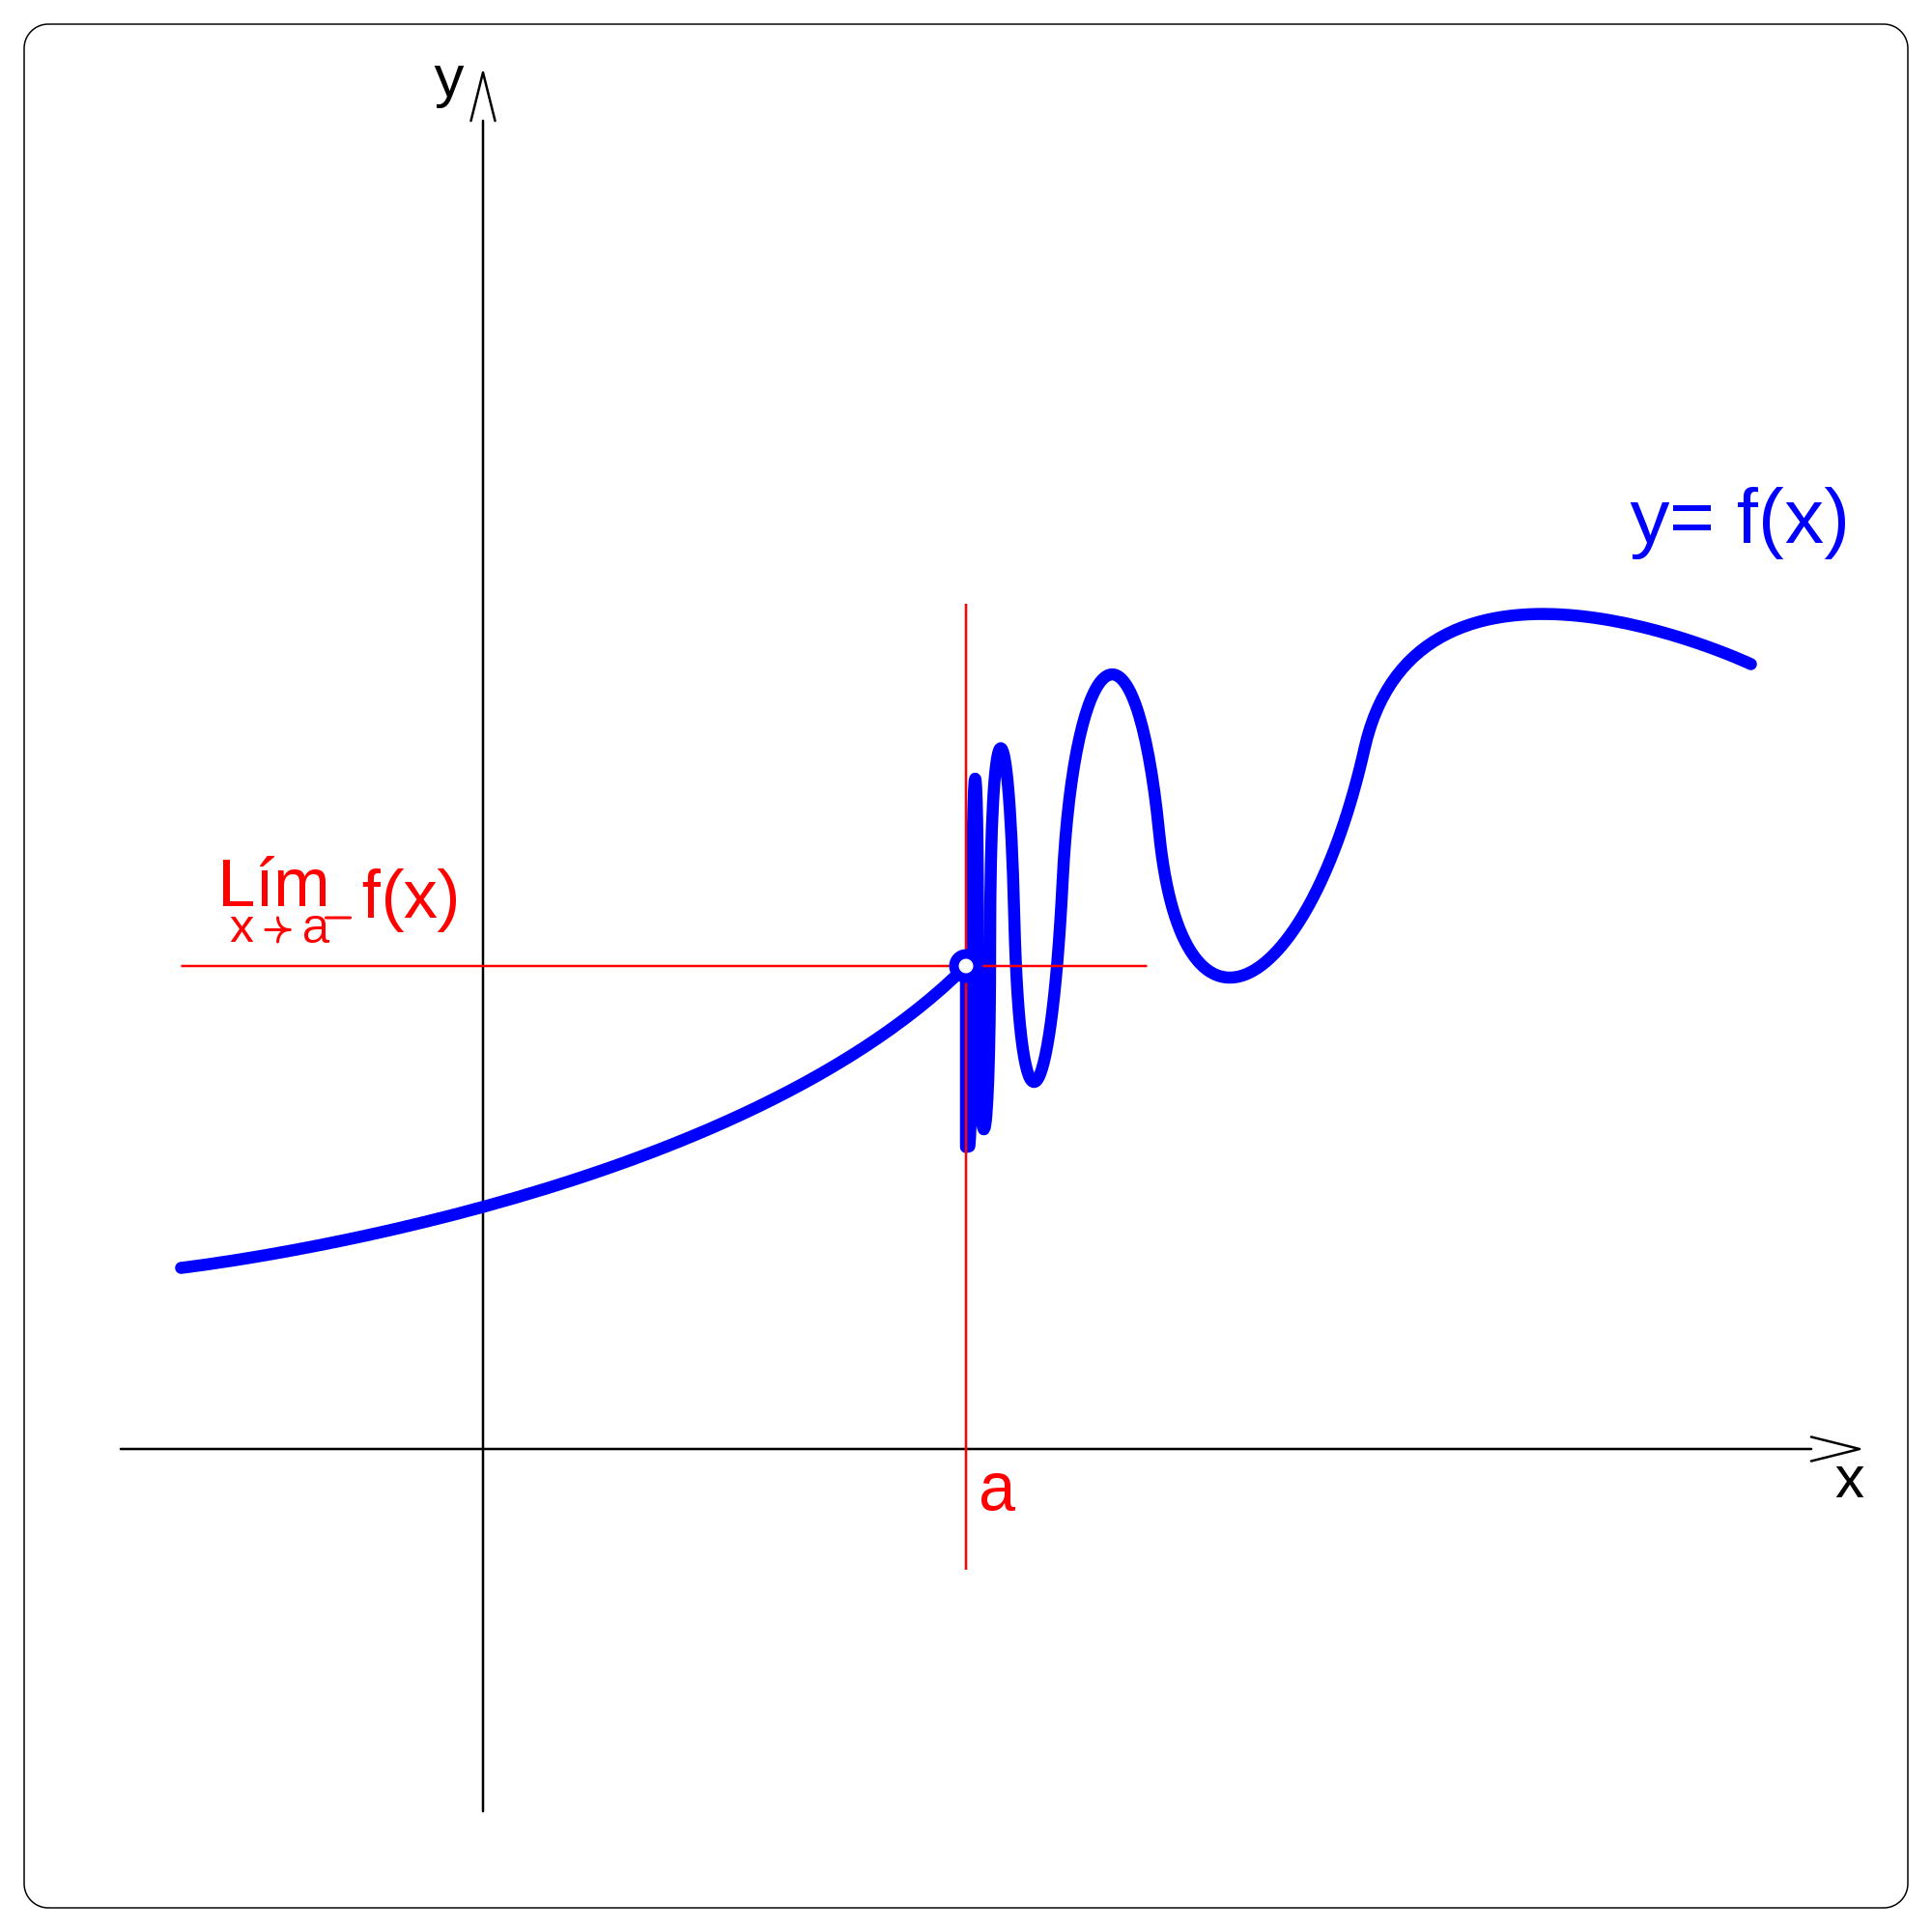
\includegraphics[scale=0.06]{img/Funs/2f3}
%\caption{Ejemplo de discontinuidad de }
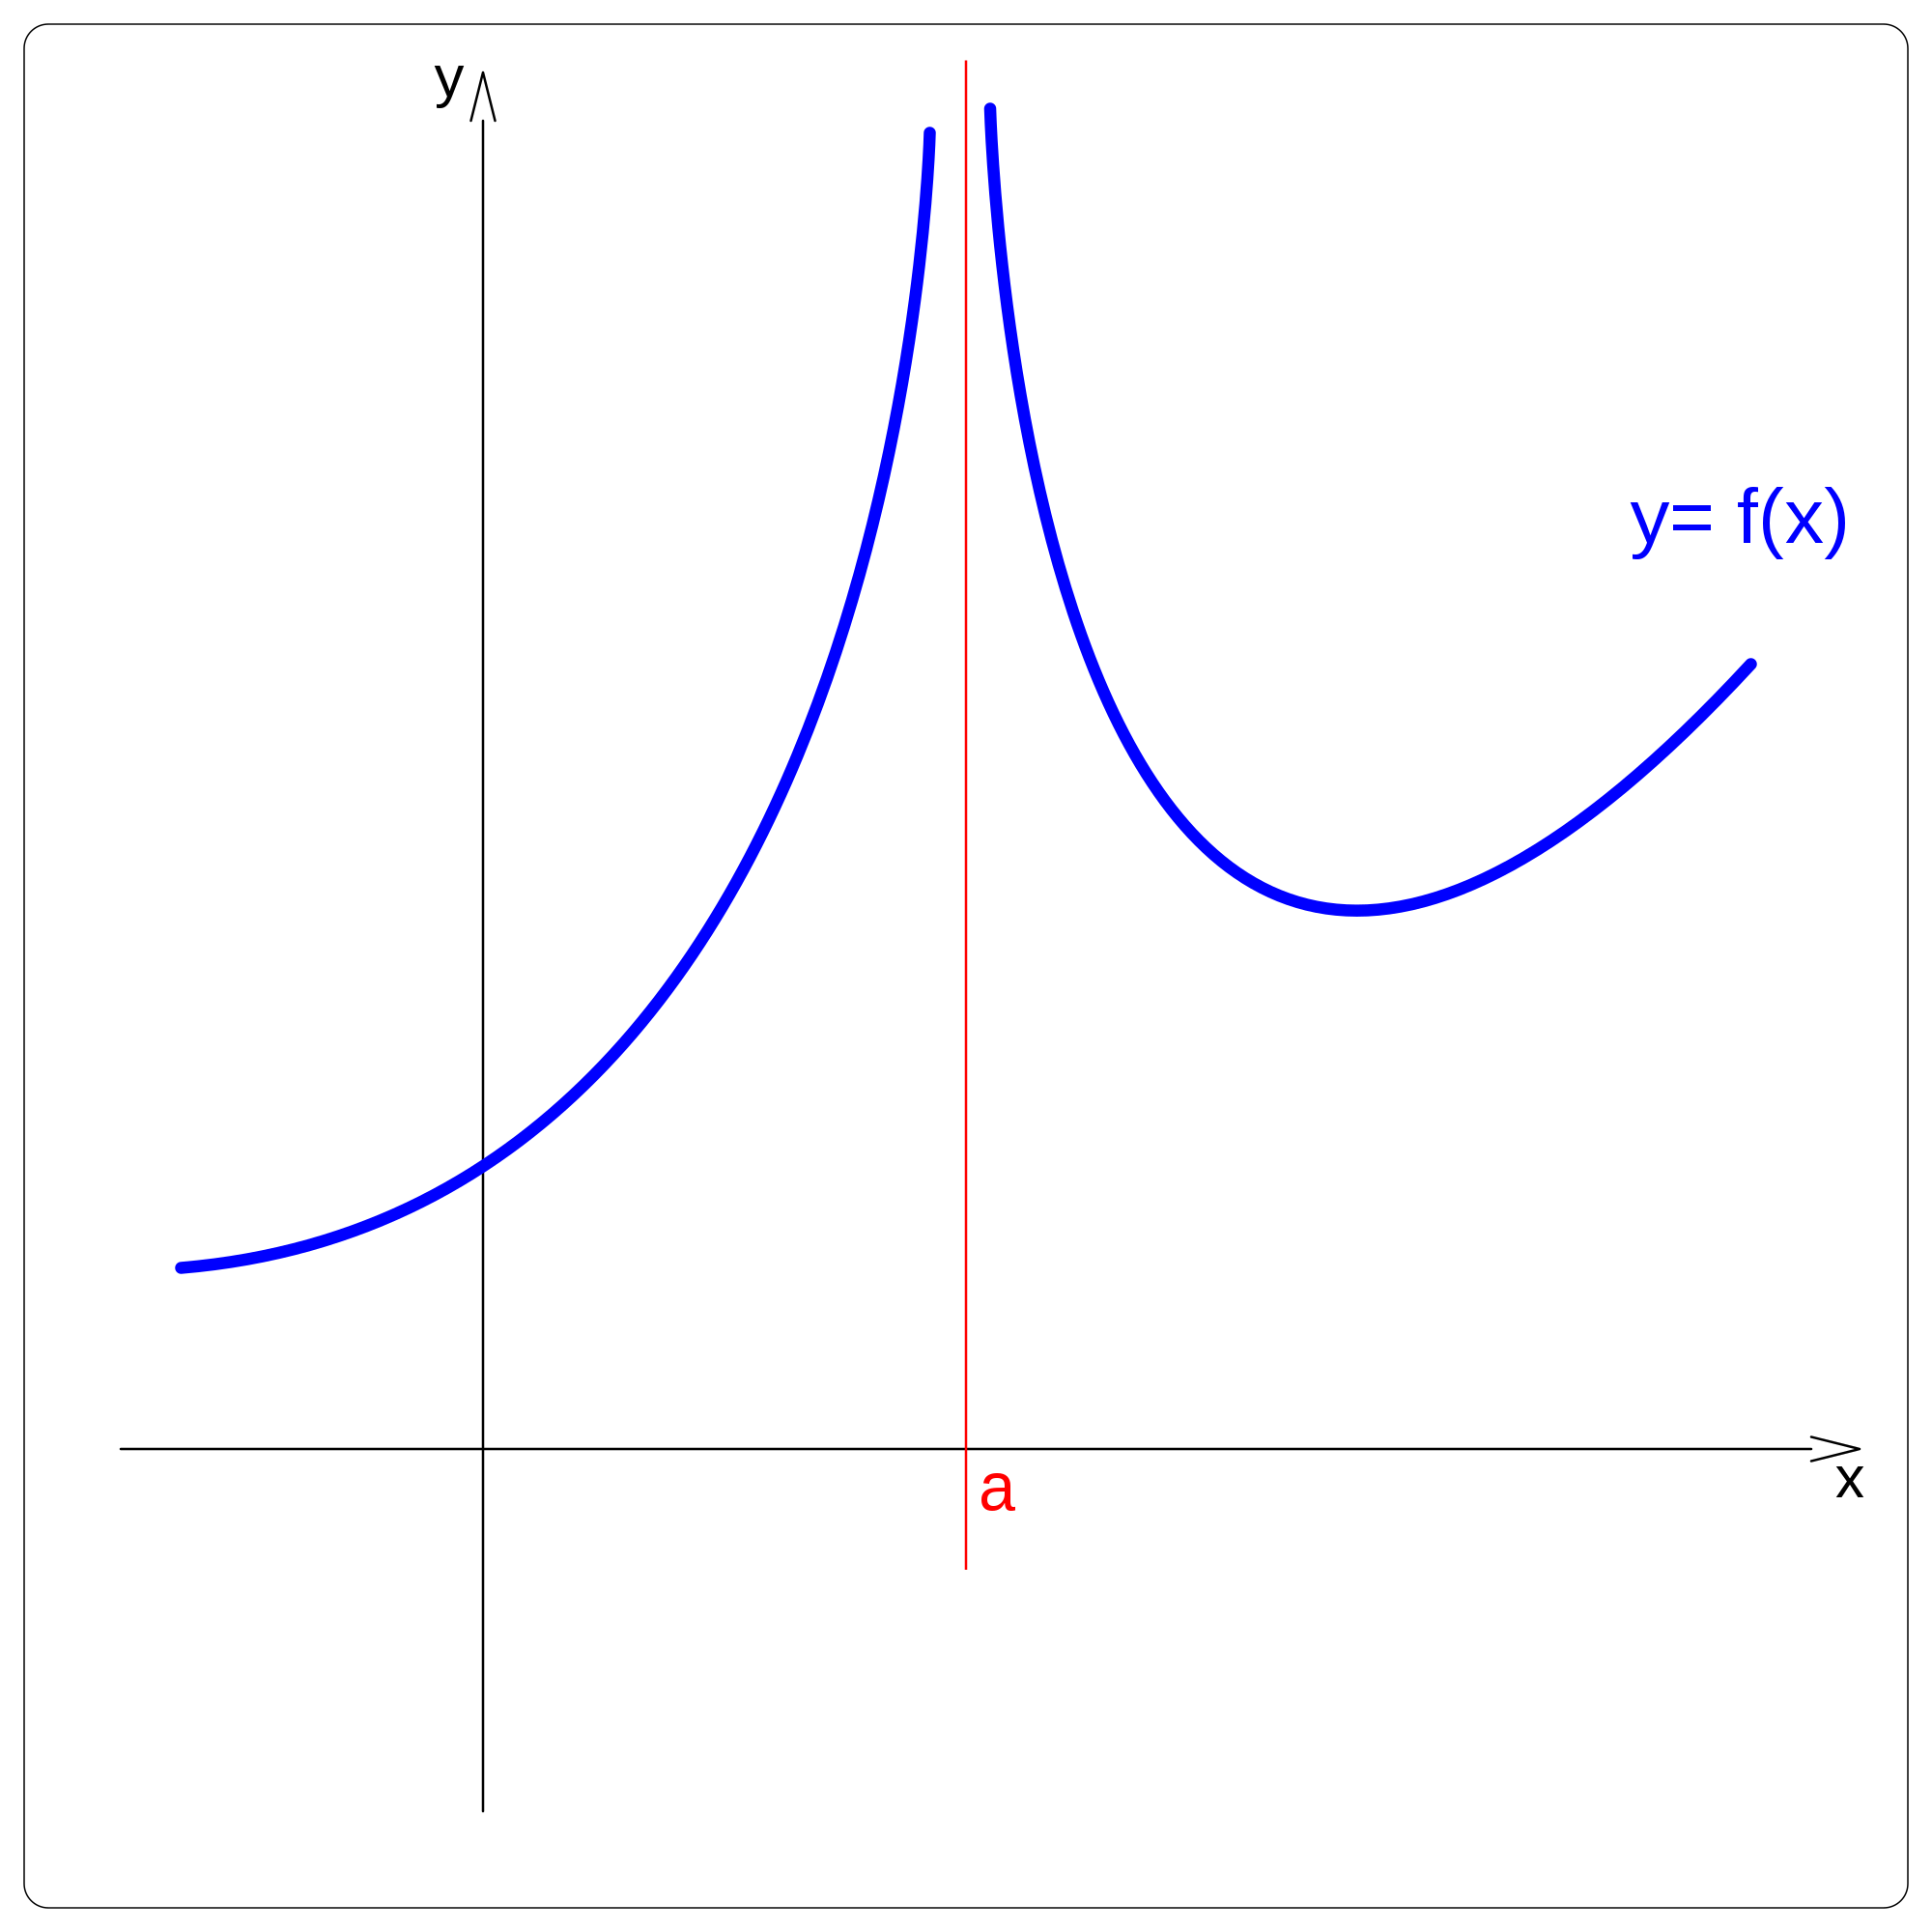
\includegraphics[scale=0.06]{img/Funs/2f4}
%\caption{Ejemplo de discontinuidad de }
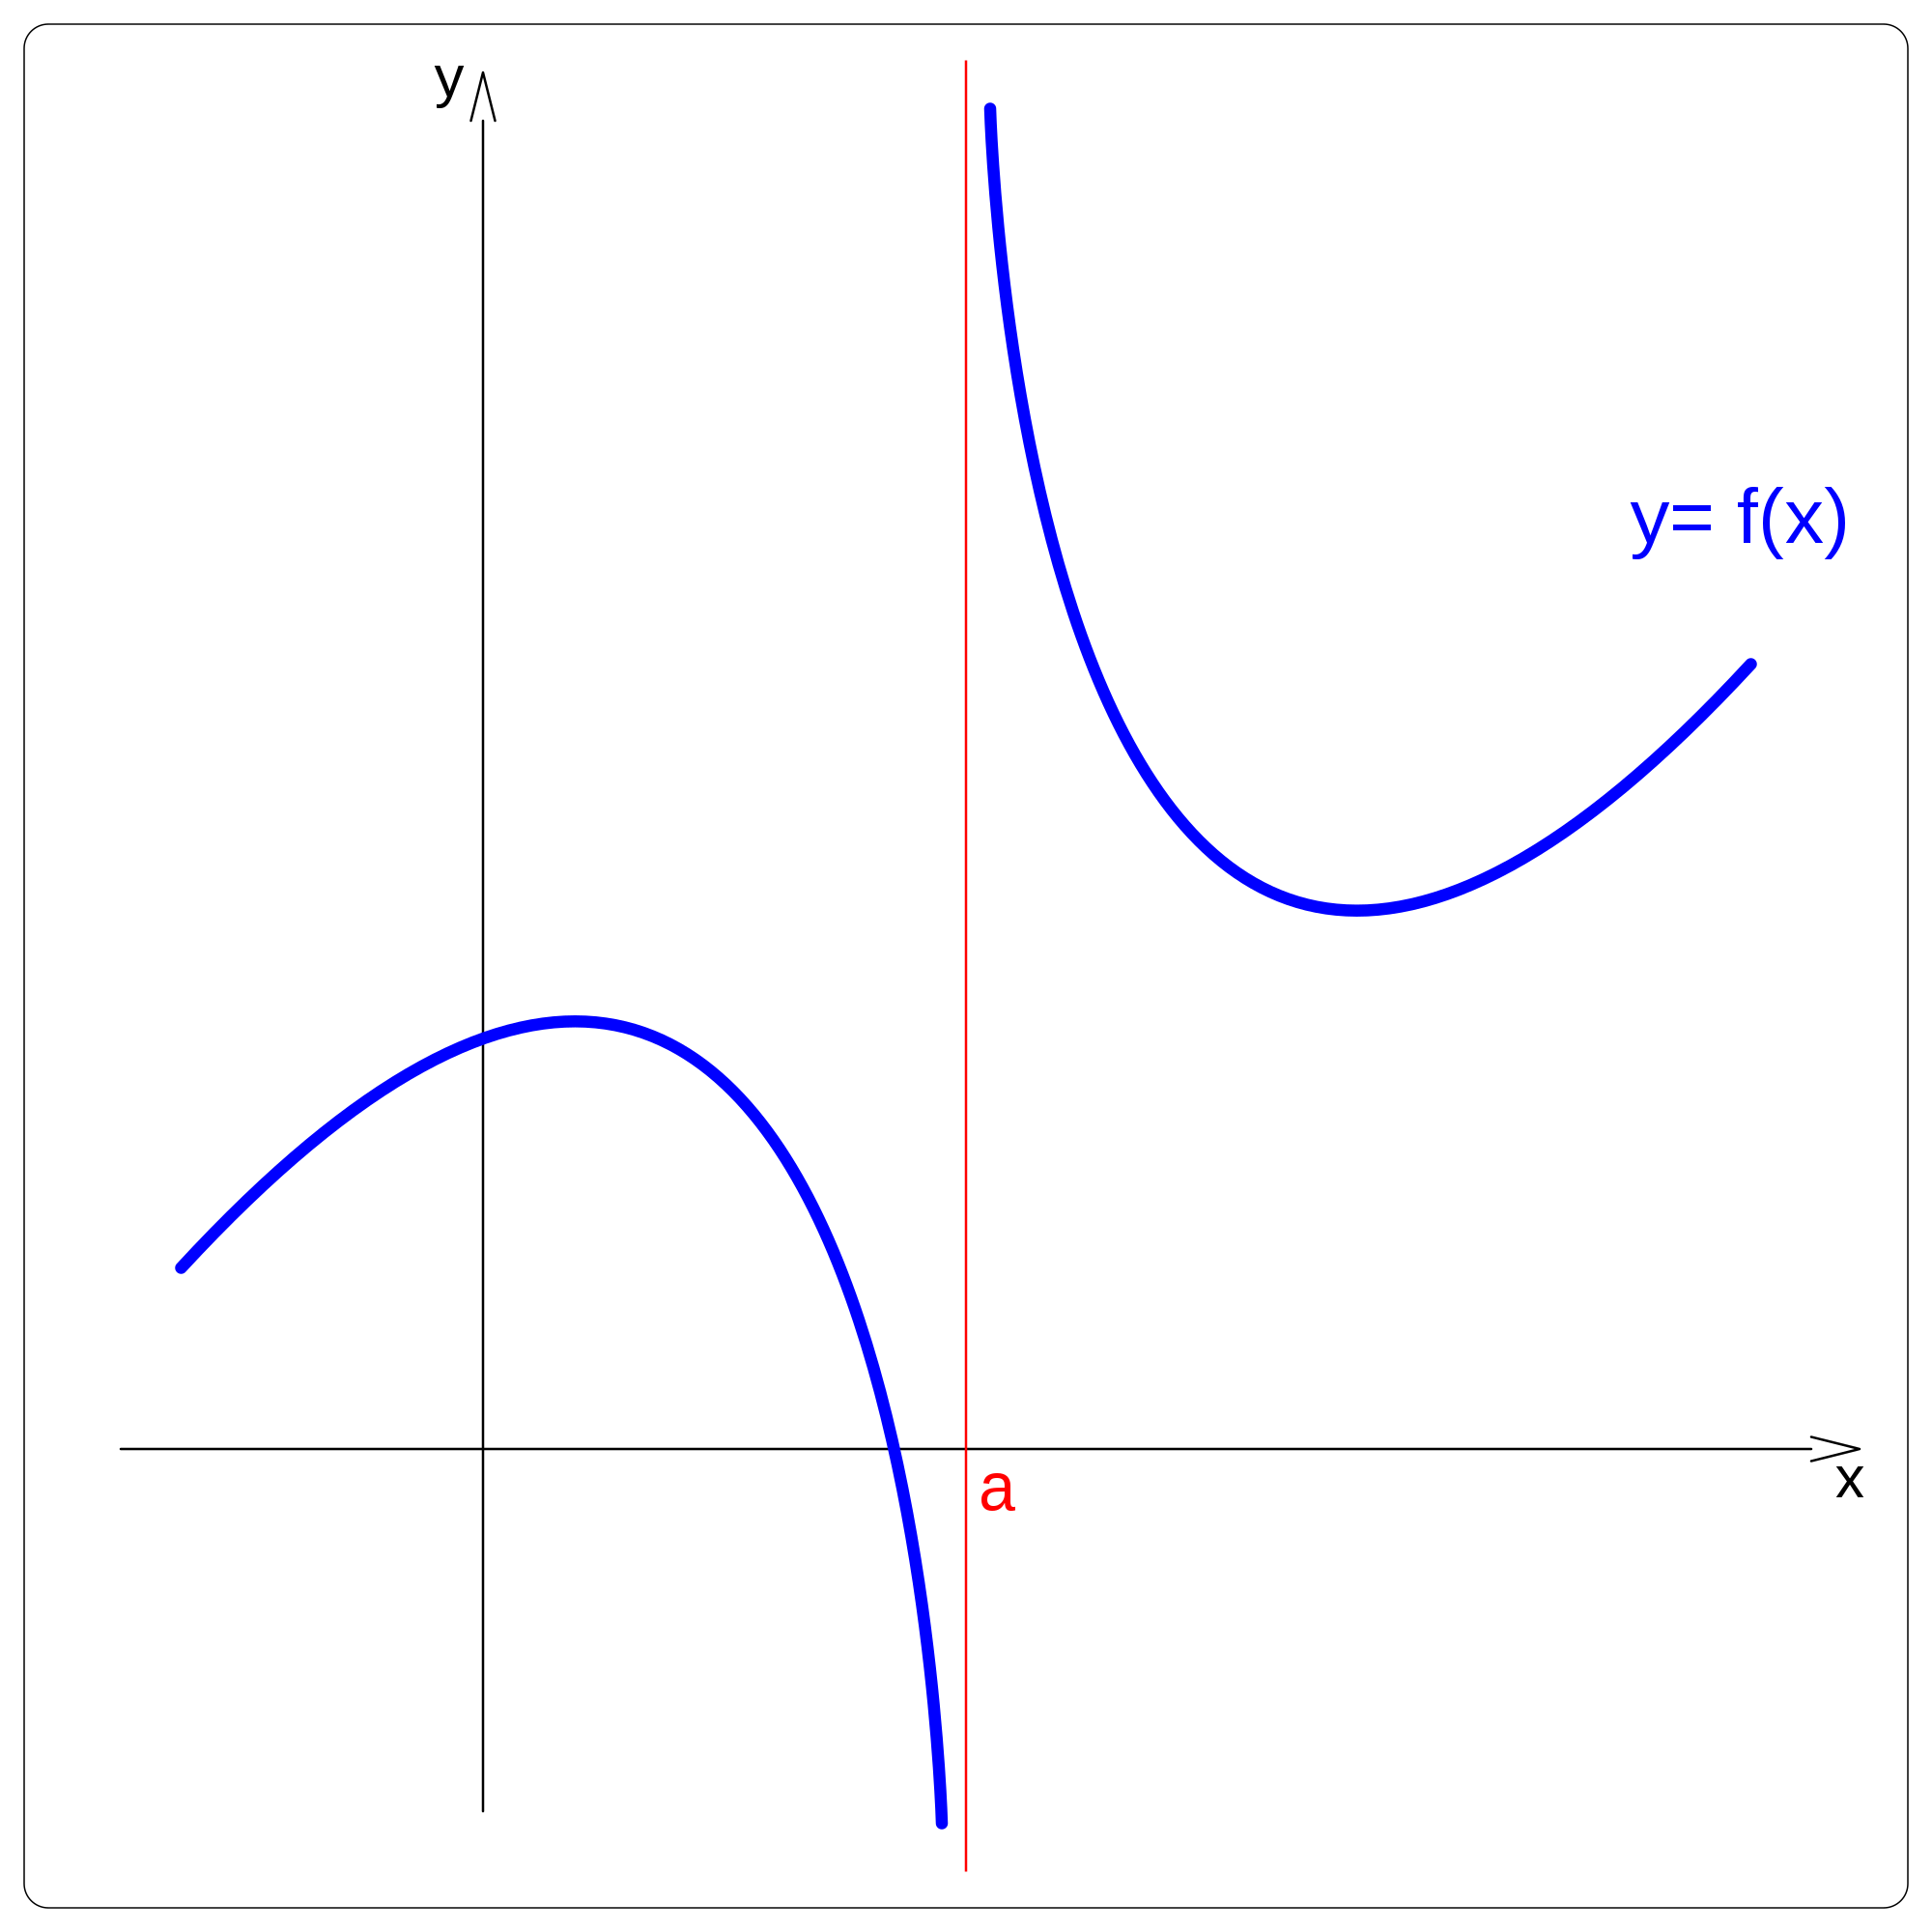
\includegraphics[scale=0.06]{img/Funs/2f5}
%\caption{Ejemplo de discontinuidad de }
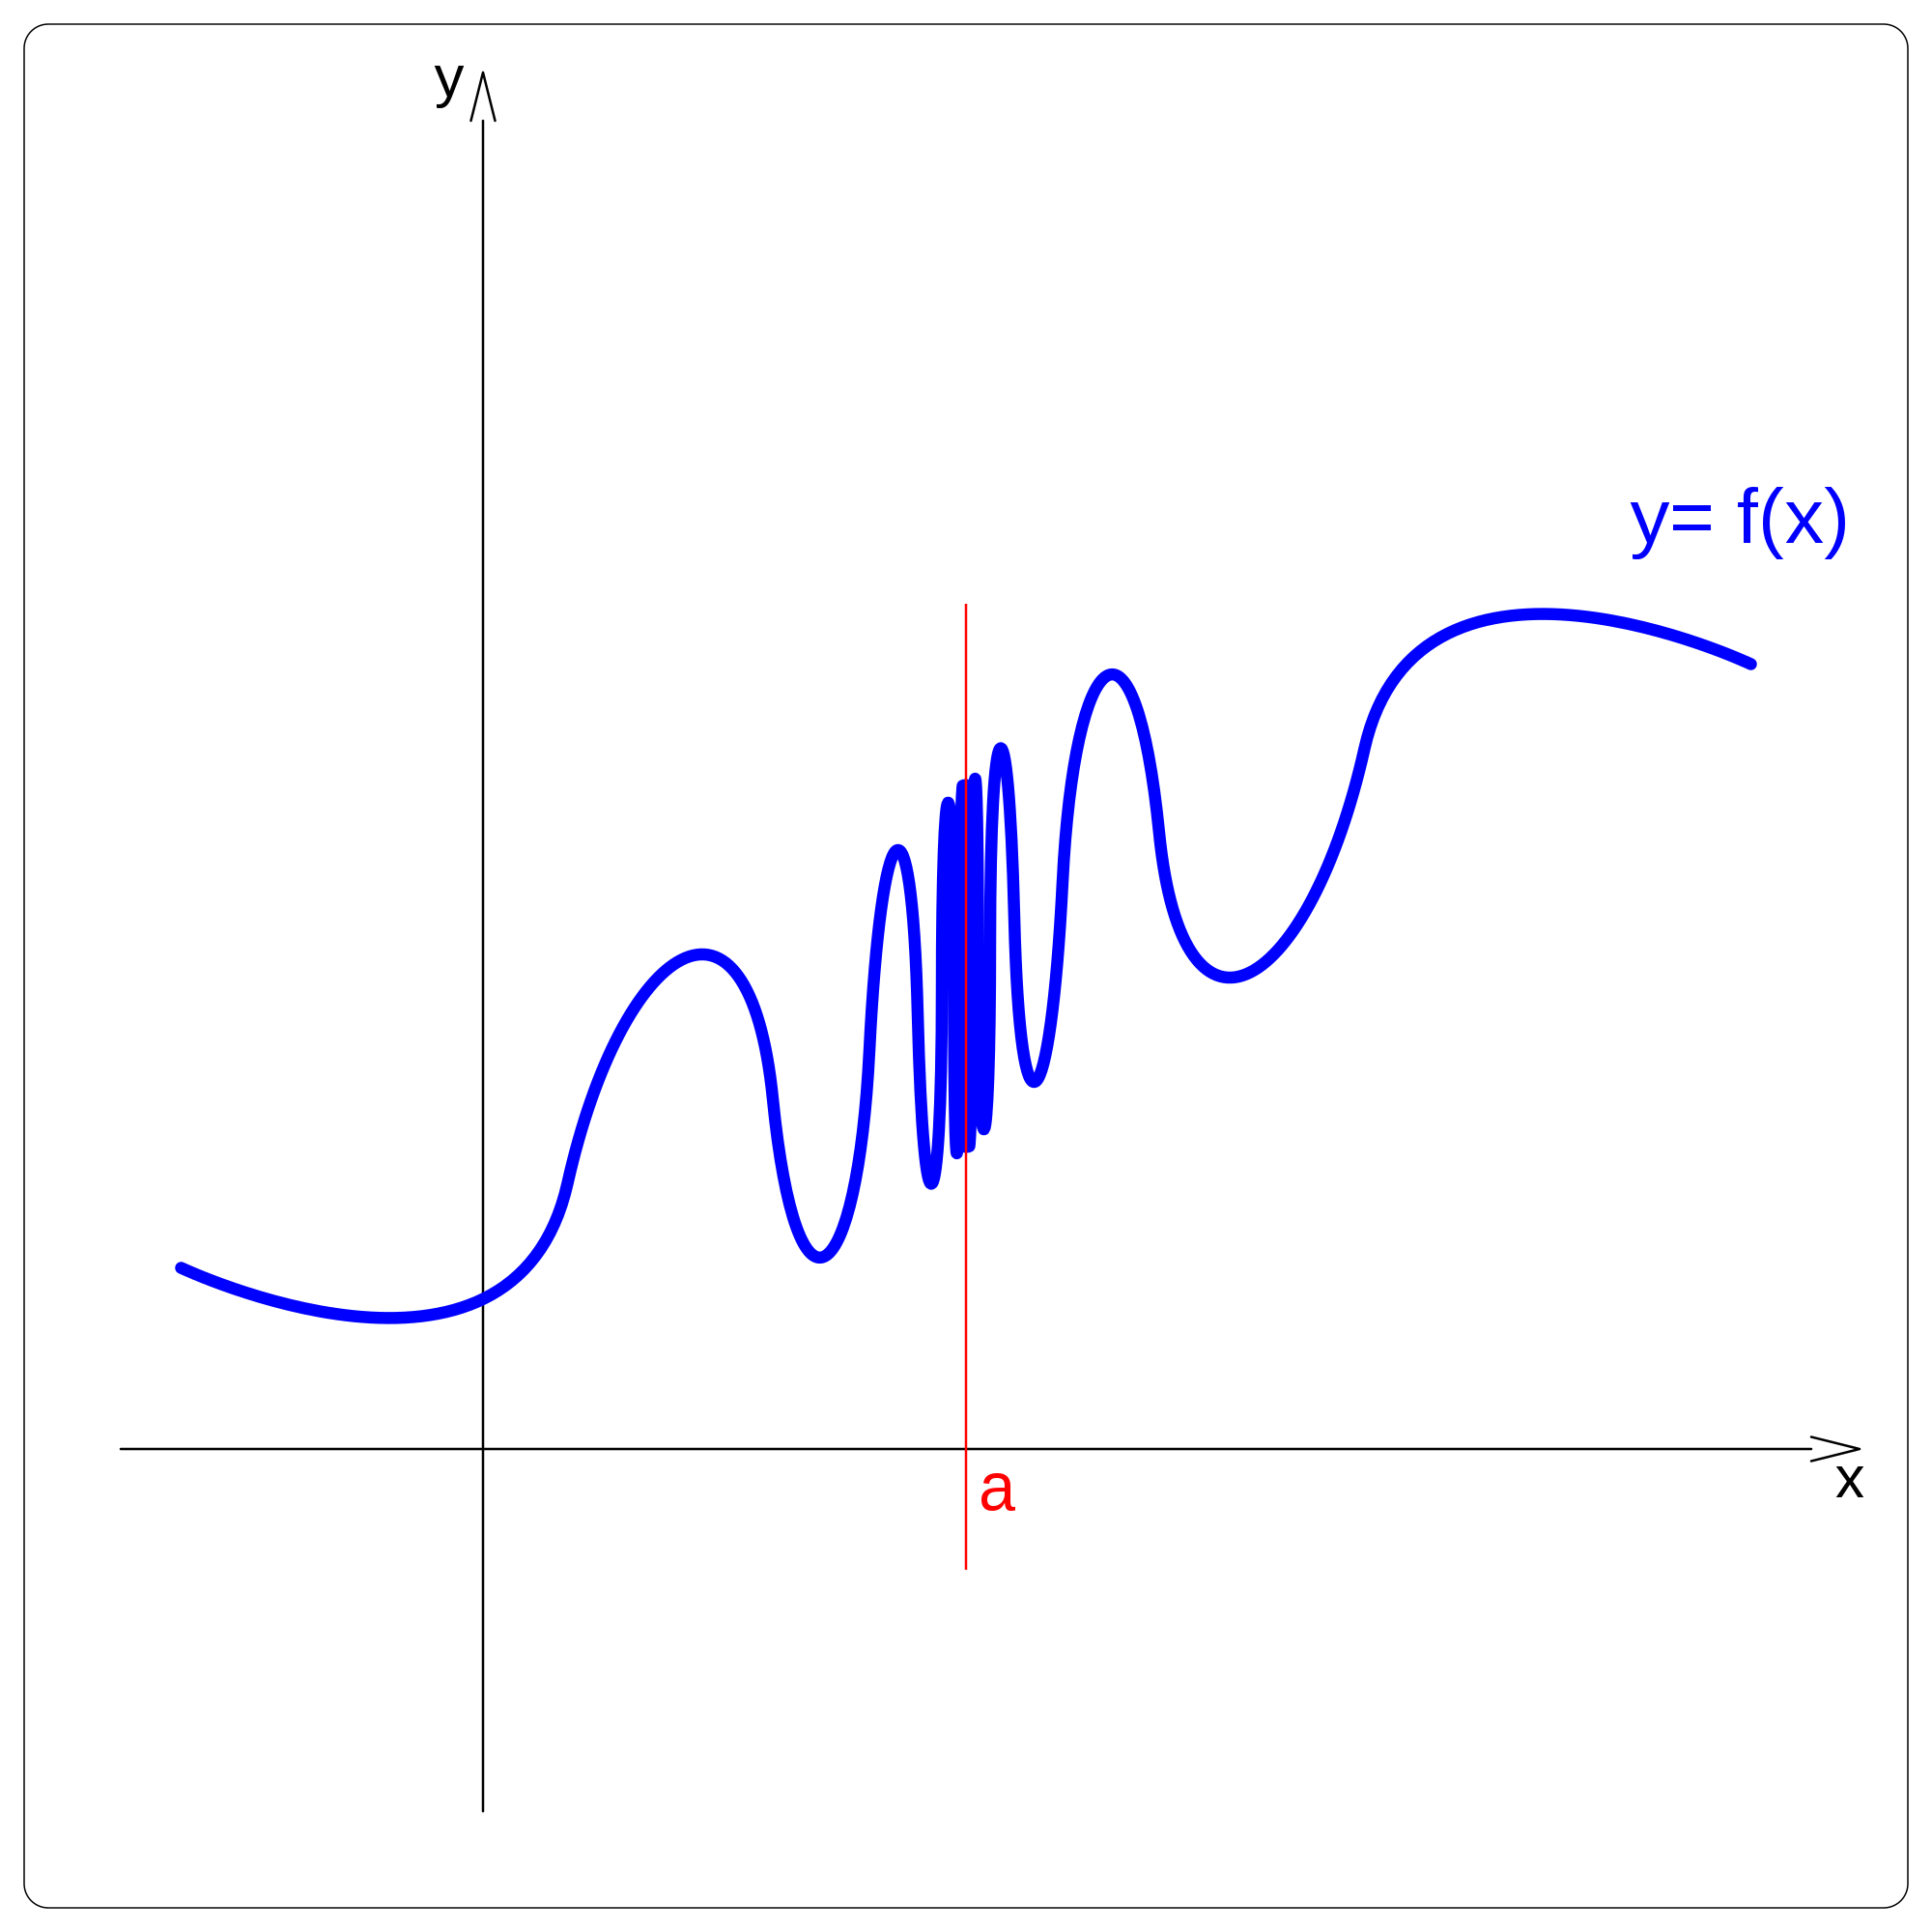
\includegraphics[scale=0.06]{img/Funs/2f6}
%\caption{Ejemplo de discontinuidad de }
%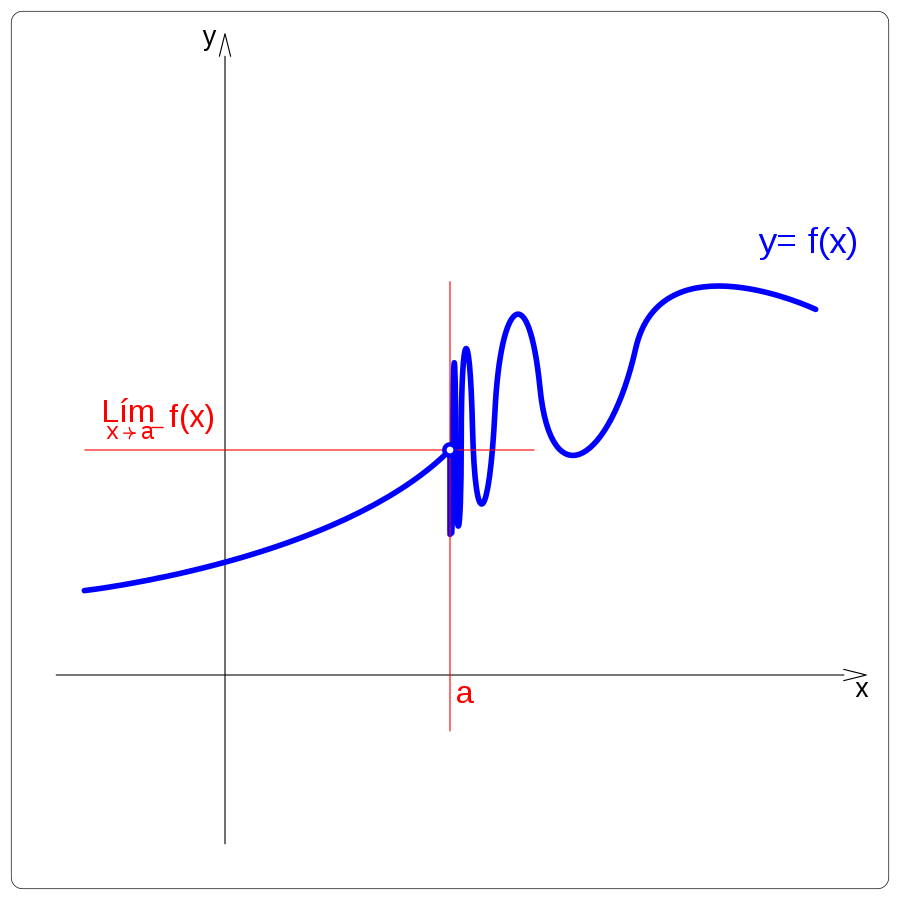
\includegraphics[scale=0.2]{img/Funs/2f7}
%\caption{Ejemplo de discontinuidad de }
\end{figure}




\begin{example}
1.  Sea la función: $f_1(x)=\left\{\begin{matrix}x^2 & \mbox{ si } x<1 \\ 0 & \mbox { para } x=1 \\ 2-x&  \mbox{ si } x>1\end{matrix}\right.$ 

El punto $x_0=1$ es una discontinuidad evitable. Esta función puede ''hacerse continua'' simplemente redefiniendo la función en este punto para que valga $f_1(1)=1$.
\end{example}

\begin{example}
2. Sea la función: $f_2(x)=\left\{\begin{matrix}x^2 & \mbox{ si } x<1 \\ 0 & \mbox { para } x=1 \\ 2-(x-1)^2& \mbox{ si } x>1\end{matrix}\right.$

El punto $x_0=1$ es una discontinuidad por salto finito.
\end{example}

\begin{example}
3. Sea la función: $f_3(x)=\left\{\begin{matrix}\sin\left(\frac{5}{x-1}\right) & \mbox{ si } x<1 \\ 0 & \mbox{ si } x=1 \\ \frac{10}{x-1}& \mbox{ si } x>1\end{matrix}\right.$

El punto $x_0=1$  una discontinuidad esencial, para lo cual hubiese bastado que uno de los dos límites laterales no exista o sea infinito (en este caso se cumple para ambos límites laterales: para el límite por izquierda y para el límite por derecha).
\end{example}

\begin{defn}[Continuidad\IS en un intervalo abierto]

	$f(x)$ es continua en $(a,b) \dimplies \forall x\in(a,b), f(x)$ es continua.
\end{defn}


\begin{defn}[Continuidad\IS por la izquierda y/o por la derecha]
	\begin{itemize}
		\item Una función $(x)$ es continua por la derecha de $a$ si $\displaystyle\lim_{x\to a^\square}f(x) = f(x)$
		\item Una función $(x)$ es continua por la izquierda de $a$ si $\displaystyle\lim_{x\to a^\square} f(x) = f(x)$
	\end{itemize}
\end{defn}

\begin{defn}[Continuidad\IS en un intervalo cerrado]

$f(x)$ es continua en $[a,b] \dimplies \forall x\in[a,b],\begin{cases} f(x) \text{ es continua en } (a,b)\\
\text{Continua por la derecha de } \square\\
\text{Continua por la izquierda de } \square\\\end{cases}$
\end{defn}
\vspace{-0.5cm}

\begin{example}
Dada $f(x) = +\sqrt{x}$.

$f(x)$ es continua en $(0,\infty)$, por ser funcion radical. 

$f(x)$ no es continua en $x=0$, ya que $\nexists\displaystyle\lim_{x\to 0^-}f(x)$. 
%
Sin embargo, sí es continua \textit{por la derecha} en $x=0$, ya que $\displaystyle\lim_{x\to 0^+} f(x) = f(x) = 0$. 

%Por lo tanto, $f(x)$ es continua en $[0,\infty)$, es decir, en su dominio.
\textbf{Conclusión:}
\end{example}

\begin{problem}
Estudia la continuidad de las siguiente funciones.
\obs Si no se indica punto para estudiar la continuidad, debe estudiarse la continuidad en $\real$

\ppart[17.2-MadA] $f(x) = \begin{cases}\displaystyle x·e^{2x} &\mbox{ si } x<0\\ \displaystyle\frac{\ln(x+1)}{x+1}&\mbox{ si } x\geq 0\end{cases}$ en $x=0$. 
\ppart[16.2-MadB] $f(x) = \begin{cases}\displaystyle\frac{1}{5-x}&\mbox{ si }x\leq0\\\displaystyle\frac{1}{5+x}&\mbox{ si }x>0\end{cases}$
\ppart[16.1-MadA] $f(x) = \begin{cases}\displaystyle\frac{\ln(1-x)}{1-x}&\mbox{ si }x<0\\\displaystyle x·e^{-x}&\mbox{ si }x\geq 0\end{cases}$
\ppart[14.2-MadB] Calcular el valor de $a$ para que $f(x)$ sea continua en $\real$, con  \[f(x) = \begin{cases}a+x·\ln(x)&\mbox{ si }x>0\\\displaystyle x^2·e^x&\mbox{ si }x\leq 0\end{cases}\]

\solution
\end{problem}